% Options for packages loaded elsewhere
\PassOptionsToPackage{unicode}{hyperref}
\PassOptionsToPackage{hyphens}{url}
\documentclass[
]{article}
\usepackage{xcolor}
\usepackage{amsmath,amssymb}
\setcounter{secnumdepth}{-\maxdimen} % remove section numbering
\usepackage{iftex}
\ifPDFTeX
  \usepackage[T1]{fontenc}
  \usepackage[utf8]{inputenc}
  \usepackage{textcomp} % provide euro and other symbols
\else % if luatex or xetex
  \usepackage{unicode-math} % this also loads fontspec
  \defaultfontfeatures{Scale=MatchLowercase}
  \defaultfontfeatures[\rmfamily]{Ligatures=TeX,Scale=1}
\fi
\usepackage{lmodern}
\ifPDFTeX\else
  % xetex/luatex font selection
\fi
% Use upquote if available, for straight quotes in verbatim environments
\IfFileExists{upquote.sty}{\usepackage{upquote}}{}
\IfFileExists{microtype.sty}{% use microtype if available
  \usepackage[]{microtype}
  \UseMicrotypeSet[protrusion]{basicmath} % disable protrusion for tt fonts
}{}
\makeatletter
\@ifundefined{KOMAClassName}{% if non-KOMA class
  \IfFileExists{parskip.sty}{%
    \usepackage{parskip}
  }{% else
    \setlength{\parindent}{0pt}
    \setlength{\parskip}{6pt plus 2pt minus 1pt}}
}{% if KOMA class
  \KOMAoptions{parskip=half}}
\makeatother
\usepackage{longtable,booktabs,array}
\usepackage{calc} % for calculating minipage widths
% Correct order of tables after \paragraph or \subparagraph
\usepackage{etoolbox}
\makeatletter
\patchcmd\longtable{\par}{\if@noskipsec\mbox{}\fi\par}{}{}
\makeatother
% Allow footnotes in longtable head/foot
\IfFileExists{footnotehyper.sty}{\usepackage{footnotehyper}}{\usepackage{footnote}}
\makesavenoteenv{longtable}
\usepackage{graphicx}
\makeatletter
\newsavebox\pandoc@box
\newcommand*\pandocbounded[1]{% scales image to fit in text height/width
  \sbox\pandoc@box{#1}%
  \Gscale@div\@tempa{\textheight}{\dimexpr\ht\pandoc@box+\dp\pandoc@box\relax}%
  \Gscale@div\@tempb{\linewidth}{\wd\pandoc@box}%
  \ifdim\@tempb\p@<\@tempa\p@\let\@tempa\@tempb\fi% select the smaller of both
  \ifdim\@tempa\p@<\p@\scalebox{\@tempa}{\usebox\pandoc@box}%
  \else\usebox{\pandoc@box}%
  \fi%
}
% Set default figure placement to htbp
\def\fps@figure{htbp}
\makeatother
% definitions for citeproc citations
\NewDocumentCommand\citeproctext{}{}
\NewDocumentCommand\citeproc{mm}{%
  \begingroup\def\citeproctext{#2}\cite{#1}\endgroup}
\makeatletter
 % allow citations to break across lines
 \let\@cite@ofmt\@firstofone
 % avoid brackets around text for \cite:
 \def\@biblabel#1{}
 \def\@cite#1#2{{#1\if@tempswa , #2\fi}}
\makeatother
\newlength{\cslhangindent}
\setlength{\cslhangindent}{1.5em}
\newlength{\csllabelwidth}
\setlength{\csllabelwidth}{3em}
\newenvironment{CSLReferences}[2] % #1 hanging-indent, #2 entry-spacing
 {\begin{list}{}{%
  \setlength{\itemindent}{0pt}
  \setlength{\leftmargin}{0pt}
  \setlength{\parsep}{0pt}
  % turn on hanging indent if param 1 is 1
  \ifodd #1
   \setlength{\leftmargin}{\cslhangindent}
   \setlength{\itemindent}{-1\cslhangindent}
  \fi
  % set entry spacing
  \setlength{\itemsep}{#2\baselineskip}}}
 {\end{list}}
\usepackage{calc}
\newcommand{\CSLBlock}[1]{\hfill\break\parbox[t]{\linewidth}{\strut\ignorespaces#1\strut}}
\newcommand{\CSLLeftMargin}[1]{\parbox[t]{\csllabelwidth}{\strut#1\strut}}
\newcommand{\CSLRightInline}[1]{\parbox[t]{\linewidth - \csllabelwidth}{\strut#1\strut}}
\newcommand{\CSLIndent}[1]{\hspace{\cslhangindent}#1}
\setlength{\emergencystretch}{3em} % prevent overfull lines
\providecommand{\tightlist}{%
  \setlength{\itemsep}{0pt}\setlength{\parskip}{0pt}}
\usepackage{bookmark}
\IfFileExists{xurl.sty}{\usepackage{xurl}}{} % add URL line breaks if available
\urlstyle{same}
\hypersetup{
  pdftitle={AURORA: Dataset Preparation and Preliminary DCGAN Feasibility for Chest Radiograph Augmentation},
  pdfauthor={Rayan Rahman; Marathwada Mitra Mandal Institute of Technology},
  hidelinks,
  pdfcreator={LaTeX via pandoc}}

\title{AURORA: Dataset Preparation and Preliminary DCGAN Feasibility for
Chest Radiograph Augmentation}
\author{Rayan Rahman \and Marathwada Mitra Mandal Institute of
Technology}
\date{Faculty review manuscript · 19 November 2026}

\begin{document}
\maketitle

\subsection{Abstract}\label{abstract}

Synthetic radiographs may help address limited training data, but
successful image generation alone does not demonstrate improved
classification. This study describes the dataset preparation and initial
execution test for AURORA, a chest radiograph augmentation project. An
inventory of 800 Shenzhen and Montgomery images was screened using a
frozen similarity audit. Excluding all 210 images involved in 206
flagged pairs left 590 images: 289 normal and 301 labelled with
tuberculosis (TB) manifestations. A stratified image-level split
allocated 413 images to training, 89 to validation and 88 to testing. A
DCGAN was trained for two epochs using 52 TB-labelled training images,
with seed 42. The run completed on an NVIDIA RTX 4050 Laptop GPU,
recording 1.32 seconds of trainer runtime and 216.92 MiB peak PyTorch
memory allocation. Both epochs produced finite losses, and the final
checkpoint passed epoch and configuration checks. The generator read
only the selected training images. This preliminary result confirms that
the selected training and recording procedure can execute on the
available hardware. It does not establish image quality, clinical
validity or a classification benefit from synthetic augmentation.

\subsection{1. Introduction}\label{introduction}

AURORA investigates whether synthetic chest radiographs can improve
classification when few TB-labelled training images are available. The
immediate task is to establish a reproducible dataset and a functioning
training procedure before undertaking the comparison. The present report
covers that preparatory stage and one short generator run.

The project uses the Shenzhen and Montgomery collections described by
Jaeger et al. (2014). Throughout this report, ``TB-labelled'' refers to
the source radiograph label, not to a diagnosis independently
established for this study. Scarcity is introduced by restricting the
positive training subset while keeping the normal training images fixed.
This experimental imbalance should not be interpreted as an estimate of
disease prevalence.

The contribution at this stage is a documented selection procedure,
controlled access to training images and an execution record that can be
checked against the code. The study does not introduce a new GAN
architecture. Whether synthetic images add useful information beyond
ordinary oversampling remains a question for subsequent experiments.

\subsection{2. Related work}\label{related-work}

DCGAN provides a convolutional baseline for adversarial image learning
(Radford et al. 2015). AURORA uses this approach as a starting point,
rather than as a method already shown to be best for the selected data.
Work on adapted latent diffusion models has also investigated chest
radiograph generation for pathological analysis (Morís et al. 2024).
Differences in model, dataset and training conditions prevent direct
comparison with this two-epoch execution test.

A useful control is to repeat real images instead of generating new
ones. Pink and Sykes found that better generative metrics did not
produce better downstream performance than count-matched real
duplication in their TB classification experiments (Pink and Sykes
2026). Their result motivates AURORA's planned duplication control; it
does not predict the outcome of this study. A systematic review likewise
documents varied quality-assessment methods and limitations in
reproducibility and bias assessment across synthetic medical-imaging
studies ({Folguera-Profitós et al.} 2026). These findings support
evaluating image quality and classification utility separately.

\subsection{3. Materials and methods}\label{materials-and-methods}

\subsubsection{3.1 Image selection}\label{image-selection}

The local inventory contains 800 images: 406 normal and 394 TB-labelled.
A pre-existing audit identified 206 potentially similar image pairs
involving 210 distinct images. The selection rule excluded every image
occurring in any flagged pair, irrespective of its label or score. All
original files and labels were preserved.

This procedure is similarity-based exclusion, not confirmation that the
excluded images are duplicates. It retained 590 images. Table 1 gives
the cohort and label counts. Exclusion rates differed substantially:
30.06\% for Shenzhen and 7.97\% for Montgomery. Selection may therefore
change the composition of the data and limit the generalizability of
later findings.

\begin{longtable}[]{@{}
  >{\raggedright\arraybackslash}p{(\linewidth - 12\tabcolsep) * \real{0.1429}}
  >{\raggedleft\arraybackslash}p{(\linewidth - 12\tabcolsep) * \real{0.1429}}
  >{\raggedleft\arraybackslash}p{(\linewidth - 12\tabcolsep) * \real{0.1429}}
  >{\raggedleft\arraybackslash}p{(\linewidth - 12\tabcolsep) * \real{0.1429}}
  >{\raggedleft\arraybackslash}p{(\linewidth - 12\tabcolsep) * \real{0.1429}}
  >{\raggedleft\arraybackslash}p{(\linewidth - 12\tabcolsep) * \real{0.1429}}
  >{\raggedleft\arraybackslash}p{(\linewidth - 12\tabcolsep) * \real{0.1429}}@{}}
\caption{Table 1. Dataset selection and image-level
allocation.}\tabularnewline
\toprule\noalign{}
\begin{minipage}[b]{\linewidth}\raggedright
Cohort and label
\end{minipage} & \begin{minipage}[b]{\linewidth}\raggedleft
Original
\end{minipage} & \begin{minipage}[b]{\linewidth}\raggedleft
Excluded
\end{minipage} & \begin{minipage}[b]{\linewidth}\raggedleft
Retained
\end{minipage} & \begin{minipage}[b]{\linewidth}\raggedleft
Train
\end{minipage} & \begin{minipage}[b]{\linewidth}\raggedleft
Validation
\end{minipage} & \begin{minipage}[b]{\linewidth}\raggedleft
Test
\end{minipage} \\
\midrule\noalign{}
\endfirsthead
\toprule\noalign{}
\begin{minipage}[b]{\linewidth}\raggedright
Cohort and label
\end{minipage} & \begin{minipage}[b]{\linewidth}\raggedleft
Original
\end{minipage} & \begin{minipage}[b]{\linewidth}\raggedleft
Excluded
\end{minipage} & \begin{minipage}[b]{\linewidth}\raggedleft
Retained
\end{minipage} & \begin{minipage}[b]{\linewidth}\raggedleft
Train
\end{minipage} & \begin{minipage}[b]{\linewidth}\raggedleft
Validation
\end{minipage} & \begin{minipage}[b]{\linewidth}\raggedleft
Test
\end{minipage} \\
\midrule\noalign{}
\endhead
\bottomrule\noalign{}
\endlastfoot
Shenzhen normal & 326 & 112 & 214 & 150 & 32 & 32 \\
Shenzhen TB-labelled & 336 & 87 & 249 & 174 & 38 & 37 \\
Montgomery normal & 80 & 5 & 75 & 53 & 11 & 11 \\
Montgomery TB-labelled & 58 & 6 & 52 & 36 & 8 & 8 \\
\textbf{Total} & \textbf{800} & \textbf{210} & \textbf{590} &
\textbf{413} & \textbf{89} & \textbf{88} \\
\end{longtable}

The selection is reproducible from the frozen reference and pair index.
The initial similarity-screening procedure and its thresholds still need
fuller documentation before a definitive effectiveness study. Retained
files have distinct exact hashes, but this does not rule out transformed
duplicates or repeated patients.

\subsubsection{3.2 Split and
preprocessing}\label{split-and-preprocessing}

Within each cohort and label stratum, filenames were sorted and shuffled
with one random generator seeded 42. Counts were allocated to a 70/15/15
target using floor rounding and the largest fractional remainders. Ties
were resolved in training, validation, test order. The resulting split
contains 413/89/88 images.

The training partition contains 203 normal and 210 TB-labelled images.
Nested positive budgets contain 52, 105 and 210 images, obtained from
one seeded ordering. The completed run used only the 52-image budget.
Patient identifiers are unavailable in the project, so disjoint image
partitions cannot be assumed to represent disjoint patients.

Generator inputs were converted to grayscale, resized to 128 × 128
pixels and normalized to {[}-1,1{]}. This resizing may discard small
radiographic findings or distort aspect ratio. High-bit-depth inputs are
rejected unless an explicit conversion is supplied.

\subsubsection{3.3 Training access and
reproducibility}\label{training-access-and-reproducibility}

Before training, the feasibility entry point checks an approval record
against hashes of the configuration, protocol, original reference, pair
audit, retained manifest, exclusion manifest and split. It reconstructs
the selection and verifies the exact ordered source IDs, effective
configuration and implementation version.

The image reader rejects unselected IDs before opening their image
files. Selected files are checked against their recorded hashes, decoded
from those same bytes and loaded into an in-memory tensor dataset. The
trainer receives these tensors rather than a directory containing the
full dataset. This is a software access control, not an operating-system
sandbox or evidence of patient-level independence.

\subsubsection{3.4 DCGAN execution test}\label{dcgan-execution-test}

The generator uses a latent dimension of 100 and generator/discriminator
widths of 64. Both networks use Adam with learning rate 0.0002 and betas
0.5 and 0.999. Training uses binary cross-entropy, full precision, one
discriminator update per generator update and gradient-norm clipping at
1.0. The discriminator's real targets are smoothed to 0.9, with fake
targets of zero; the generator's target is one.

The run uses seed 42 and two epochs. With 52 images and batch size 16,
each epoch contains batches of 16, 16, 16 and 4 images. The reported
epoch loss is the arithmetic mean of the four batch losses, rather than
an image-weighted mean. The final checkpoint is retained without
quality-based selection. No classifier is fitted and no holdout
evaluation is performed in this test.

\subsection{4. Results}\label{results}

The two-epoch run completed on an NVIDIA GeForce RTX 4050 Laptop GPU.
Its recorded read-ID list matched the 52 selected TB training images,
with no validation/test overlap. The final checkpoint passed the
required epoch and configuration checks. Table 2 reports the execution
measurements.

\begin{longtable}[]{@{}lr@{}}
\caption{Table 2. Measurements from the single feasibility
run.}\tabularnewline
\toprule\noalign{}
Measurement & Observed value \\
\midrule\noalign{}
\endfirsthead
\toprule\noalign{}
Measurement & Observed value \\
\midrule\noalign{}
\endhead
\bottomrule\noalign{}
\endlastfoot
Trainer runtime & 1.3219 s \\
Total entry-function runtime & 6.1937 s \\
Peak PyTorch allocated GPU memory & 216.92 MiB \\
Peak PyTorch reserved GPU memory & 282.00 MiB \\
Generator mean loss, epochs 1 / 2 & 0.6178 / 0.4872 \\
Discriminator mean loss, epochs 1 / 2 & 0.3908 / 0.1918 \\
\end{longtable}

Total timing excludes interpreter and import startup. Trainer timing
includes its checkpoint and sample-output operations. Memory values
describe PyTorch's allocator, not the total GPU footprint. Only one run
was measured; no confidence interval or estimate of full-study runtime
is inferred.

\begin{figure}
\centering
\pandocbounded{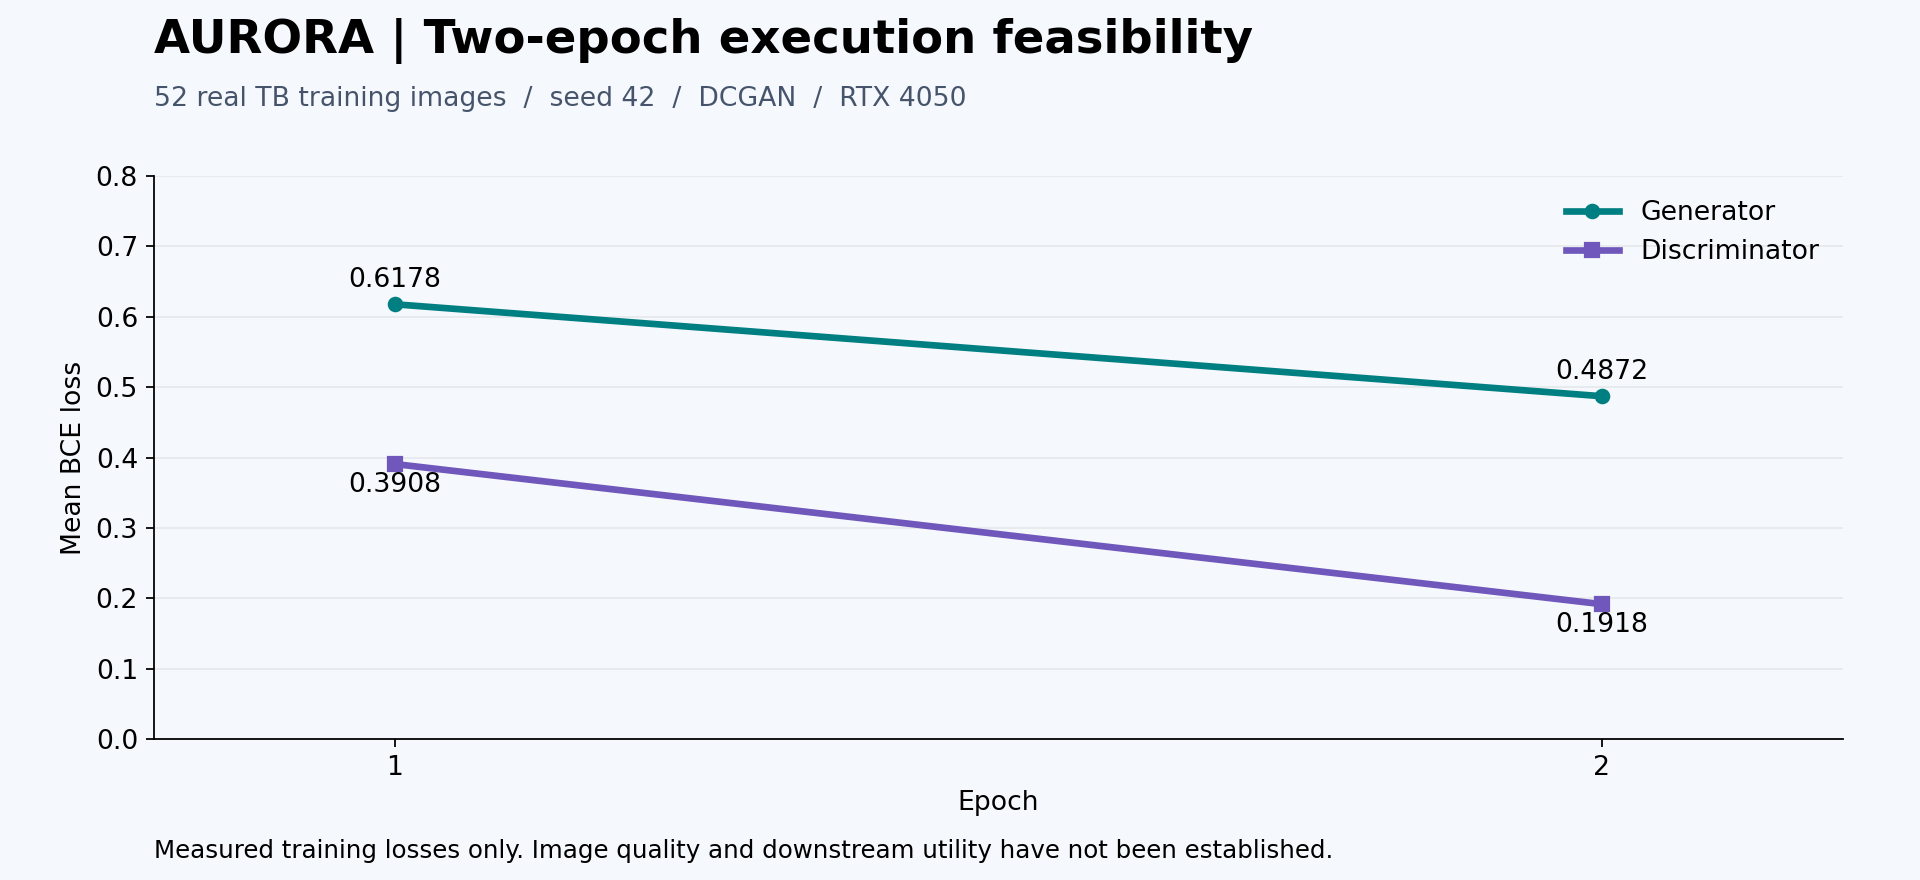
\includegraphics[keepaspectratio,alt={Figure 1. Recorded epoch losses for 52 TB-labelled training images. Lines connect the two observations; declining loss alone does not establish convergence, diversity or diagnostic fidelity.}]{../../docs/images/feasibility-losses.png}}
\caption{Figure 1. Recorded epoch losses for 52 TB-labelled training
images. Lines connect the two observations; declining loss alone does
not establish convergence, diversity or diagnostic fidelity.}
\end{figure}

Both epoch losses were finite. There are no measured classifier scores,
generative-quality scores or clinical-reader assessments from this run.
The result supports execution feasibility under the stated
configuration, rather than effectiveness of synthetic augmentation.

\subsection{5. Discussion}\label{discussion}

The run provides a limited but useful development milestone: the
selected training images can pass through the approval, preprocessing,
optimization and checkpoint-recording procedure on the available GPU.
That is sufficient to proceed with further evaluation, but not to
conclude that the generated images are useful for TB classification.

Several limitations remain. Automated exclusion may remove valid images
and leave unidentified near-duplicates. Its different rates across
cohorts may introduce selection bias. Source labels were not
independently clinically revalidated, and missing patient identifiers
prevent assurance of patient-independent evaluation. The low image
resolution and brief training duration also preclude conclusions about
anatomical quality, memorization or longer-run stability.

The Montgomery validation and test partitions each contain 19 images,
including eight TB-labelled images. One TB error would change subgroup
recall by 12.5 percentage points. Later cohort-level results will need
to report these small denominators and their uncertainty.

\subsubsection{Further work}\label{further-work}

The next stage will compare real-only training, repeated real TB images,
mild conventional augmentation of TB images, and DCGAN-generated TB
images. The repeated-real and synthetic conditions will add the same
number of images at each positive-data budget. Conventional augmentation
will exclude horizontal flipping. Classifier optimization budgets and
real evaluation partitions will be held fixed. These comparisons have
not yet been run; the detailed settings and remaining implementation
work are documented in the repository. Their purpose is to measure
whether synthesis adds value beyond simpler alternatives, including when
the result is negative or inconclusive.

\subsection{6. Conclusion}\label{conclusion}

AURORA has completed dataset preparation and one reproducible DCGAN
execution test using 52 TB-labelled training images. The run produced
finite losses and a checkpoint consistent with the specified two-epoch
configuration, without generator access to holdout images. These
findings establish preliminary execution feasibility. The effect of
synthetic augmentation on classification remains to be measured.

\subsection{Code and writing
acknowledgment}\label{code-and-writing-acknowledgment}

Code, protocol and run documentation are available at
\href{https://github.com/xt67/AURORA}{github.com/xt67/AURORA} under
Apache 2.0; dataset and model redistribution rights are separate. The
execution used commit \texttt{032adc2}. Exact hashes and local artifact
locations are recorded in the repository's feasibility report. No
clinical or institutional approval is asserted by this technical report.

Codex and Paper Orchestra assisted with outlining, drafting and language
editing. Numerical findings were drawn from the recorded experiment
artifacts. This version is submitted for faculty review.

\section*{References}\label{bibliography}
\addcontentsline{toc}{section}{References}

\protect\phantomsection\label{refs}
\begin{CSLReferences}{1}{1}
\bibitem[\citeproctext]{ref-folguera2026}
{Folguera-Profitós, Júlia et al.} 2026. {``Quality Assessment and Model
Training Impact of Synthetic Images in Medical Diagnostic Imaging:
Systematic Review.''} \emph{JMIR AI} 5: e81472.
\url{https://doi.org/10.2196/81472}.

\bibitem[\citeproctext]{ref-jaeger2014}
Jaeger, Stefan, Sema Candemir, Sameer Antani, Yi-Xiang J. Wang, Pu-Xuan
Lu, and George Thoma. 2014. {``Two Public Chest x-Ray Datasets for
Computer-Aided Screening of Pulmonary Diseases.''} \emph{Quantitative
Imaging in Medicine and Surgery} 4 (6): 475--77.
\url{https://doi.org/10.3978/j.issn.2223-4292.2014.11.20}.

\bibitem[\citeproctext]{ref-moris2024}
Morís, Daniel I., Joaquim de Moura, Jorge Novo, and Marcos Ortega. 2024.
{``Adapted Generative Latent Diffusion Models for Accurate Pathological
Analysis in Chest x-Ray Images.''} \emph{Medical \& Biological
Engineering \& Computing} 62: 2189--212.
\url{https://doi.org/10.1007/s11517-024-03056-5}.

\bibitem[\citeproctext]{ref-pink2026}
Pink, Connor, and Ed Sykes. 2026. {``Disentangling Dataset Size from
Synthetic Diversity in Tuberculosis Chest x-Ray Classification.''}
\emph{Proceedings of the 39th Canadian Conference on Artificial
Intelligence}, Proceedings of machine learning research, vol. 318:
954--61. \url{https://proceedings.mlr.press/v318/pink26a.html}.

\bibitem[\citeproctext]{ref-radford2015}
Radford, Alec, Luke Metz, and Soumith Chintala. 2015. \emph{Unsupervised
Representation Learning with Deep Convolutional Generative Adversarial
Networks}. arXiv:1511.06434. \url{https://arxiv.org/abs/1511.06434}.

\end{CSLReferences}

\end{document}
